\section{格式化输出}

\begin{frame}[fragile]\ft{\secname}
\begin{table}
\centering
\caption{格式说明符}
\begin{tabular}{p{2.5cm}|p{7.5cm}} \hline
格式说明符 & ~~~~~~~~输出 \\ \hline\hline 
 \lstinline|%a| & 浮点数、十六进制和p-计数法 \\
 \lstinline|%A| & 浮点数、十六进制和P-计数法 \\
 \lstinline|%c| & 一个字符\\
 \lstinline|%d| & 有符号十进制数\\\hline
\end{tabular}
\end{table}
\end{frame}


\begin{frame}[fragile]\ft{\secname}
\begin{table}
\centering
\caption{格式说明符}
\begin{tabular}{p{2.5cm}|p{7.5cm}} \hline
格式说明符 & ~~~~~~~~输出 \\ \hline\hline 
 \lstinline|%e| & 浮点数、e-计数法\\
 \lstinline|%E| & 浮点数、E-计数法\\
 \lstinline|%f| & 浮点数、十进制计数法\\
 \lstinline|%g| & 根据数值不同自动选\lstinline|%f|或\lstinline|%e|。\lstinline|%e|格式在指数小于-4或大于等于精度时使用\\
 \lstinline|%G| & 根据数值不同自动选\lstinline|%f|或\lstinline|%E|。\lstinline|%E|格式在指数小于-4或大于等于精度时使用\\\hline
\end{tabular}
\end{table}
\end{frame}

\begin{frame}[fragile]\ft{\secname}
\begin{table}
\centering
\caption{格式说明符}
\begin{tabular}{p{2.5cm}|p{7.5cm}} \hline
格式说明符 & ~~~~~~~~输出 \\ \hline\hline 
\lstinline|%i| & 有符号十进制整数(同\lstinline|%d|)\\
\lstinline|%o| & 无符号八进制整数\\
\lstinline|%p| & 指针\\
\lstinline|%s| & 字符串\\\hline
\end{tabular}
\end{table}
\end{frame}


\begin{frame}[fragile]\ft{\secname}
\begin{table}
\centering
\caption{格式说明符}
\begin{tabular}{p{2.5cm}|p{7.5cm}} \hline
格式说明符 & ~~~~~~~~输出 \\ \hline\hline 
\lstinline|%x| & 使用十六进制数字0-f的无符号十六进制整数\\
\lstinline|%X| & 使用十六进制数字0-F的无符号十六进制整数\\
\hline
\end{tabular}
\end{table}
\end{frame}

\begin{frame}[fragile]\ft{\secname}
\begin{lstlisting}[title=printf的使用格式]
printf(Control-string, item1, item2, ...);
\end{lstlisting} \vspace{0.1in}

\begin{itemize}
\item item1, item2等是要打印的项目,它们可以是变量,也可以是常量,甚至是在打印之前进行计算的表达式。\\[0.1in]
\item 控制字符串(Control-string)是一个描述项目如何打印的字符串,它为每个要打印的项目包含一个格式说明符。

\end{itemize}
\end{frame}

\begin{frame}[fragile]\ft{\secname}
\begin{figure}
\centering
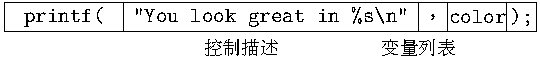
\includegraphics[]{ch04/images/printf.pdf}
\end{figure}

\vspace{.1in} \pause 

\red{不要忘记给控制字符串后面的列表中的每个项目都使用一个格式说明符。}
\end{frame}

\begin{frame}[fragile]\ft{\secname}
\begin{itemize}
\item 如果只打印一个语句,则不需要任何格式说明符;\\[0.1in]
\item 如果只打印数据,则无须加入任何说明内容。\\[0.1in]
\item 想打印\lstinline|%|,必须使用两个\lstinline|%%|符号。
\end{itemize}

\begin{lstlisting}
printf("Once more you open the door!\n");
printf("%s%d\n", "area = ", area);
printf("%d%% = %f\n", 30, 0.3);
\end{lstlisting}
\end{frame}

\begin{frame}[fragile]\ft{\secname: \lstinline|\%d|}
\begin{itemize}
\item \lstinline|%d|:  按整型数据的实际长度输出\\[0.1in]
\item \lstinline|%md|:  输出字段的宽度为m,右对齐\\ 
\item[] 若数据位数<m,左端补空格;若>=m,按实际位数输出。\\[0.1in]
\item \lstinline|%-md|: 输出字段的宽度为m,左对齐\\ 
\item[] 若数据位数<m,右端补空格;若>=m,按实际位数输出。\\[0.1in]
\item \lstinline|%0md|: 输出字段的宽度为m,右对齐 \\ 
\item[] 若数据位数<m,右端补0;若>=m,按实际位数输出。
\end{itemize}
\end{frame}

\begin{frame}[fragile]\ft{\secname: \lstinline|\%d|}
\lstinputlisting[language=c,frame=single,numbers=left]{ch04/code/width.c}
\end{frame}

\begin{frame}[fragile]\ft{\secname: \lstinline|\%d|}
\begin{lstlisting}[showspaces=true,backgroundcolor=\color{red!20}]
*1000*
*1000*
*      1000*
*1000      *
*0000001000*
\end{lstlisting}
\end{frame}


\begin{frame}[fragile,allowframebreaks]\ft{\secname: \lstinline|\%f|、\lstinline|\%e|和\lstinline|\%E|}
\lstinputlisting[language=c,numbers=left]
{ch04/code/floats.c}
\end{frame}

\begin{frame}[fragile]\ft{\secname: \lstinline|\%f|、\lstinline|\%e|和\lstinline|\%E|}
\begin{lstlisting}[showspaces=true,backgroundcolor=\color{red!20}]
*3852.990000*
*3.852990e+03*
*3852.99*
*3853.0*
*  3852.990*
* 3.853e+03*
* 3.853E+03*
*+3852.99*
*3852.99   *
*0003852.99*
\end{lstlisting}
\end{frame}

\begin{frame}[fragile]\ft{\secname: \lstinline|\%f|、\lstinline|\%e|和\lstinline|\%E|}
\begin{lstlisting}[backgroundcolor=\color{red!20}]
%m.nf     %m.ne      %m.nE
\end{lstlisting}

\begin{itemize}
\item m:字段宽度
\item n:小数点后面数字的个数
\end{itemize}
\end{frame}

\begin{frame}[fragile]\ft{\secname: \lstinline|\%f|、\lstinline|\%e|和\lstinline|\%E|}
\begin{lstlisting}[backgroundcolor=\color{red!20}] 
%.nf
\end{lstlisting}

\begin{itemize}
\item  整数部分以实际长度输出
\item n:小数点后面数字的个数
\end{itemize}
\end{frame}

\begin{frame}[fragile]\ft{\secname: \lstinline|\%f|、\lstinline|\%e|和\lstinline|\%E|}
\begin{lstlisting}[backgroundcolor=\color{red!20}] 
%m.f
\end{lstlisting}

\begin{itemize}
\item m: 字段宽度
\item 不输出小数点后的数字
\end{itemize}
\end{frame}

\begin{frame}[fragile]\ft{\secname: \lstinline|\%d|}
    \lstinputlisting[language=c,numbers=left]{ch04/code/flags.c}    
\end{frame}

\begin{frame}[fragile]\ft{\secname: \lstinline|\%d|}
\begin{lstlisting}[showspaces=true,backgroundcolor=\color{red!20}]
1f 1F 0x1f 0X1F
*42*
* 42*
*-42*
*    6*
*  006*
*00006*
*  006*
\end{lstlisting}
\end{frame}


\begin{frame}[fragile] \ft{\secname: \lstinline|\%d|}
 使用\lstinline|% d|在正值之前产生一个前导空格,在负值之前不产生前导空格。
这使得有效位相同的正值和负值以相同字段宽度打印输出。
\end{frame}

\begin{frame}[fragile]\ft{\secname: \lstinline|\%d|} 
\begin{itemize}
\item \lstinline|%5.3d|为精度说明符,用于在整数格式中来产生足够的前导零以填满要求的最小数字位数。\\[0.1in]
\item \lstinline|%05d|将会用前导零填满整个字段宽度。\\[0.1in]
\item 在\lstinline|%05.3d|中,0标志和精度说明符同时出现,此时0标志将会忽略。
\end{itemize}
\end{frame}

\begin{frame}[fragile]\ft{\secname: \lstinline|\%s|}
\lstinputlisting[language=c,,numbers=left]{ch04/code/strings.c}    
\end{frame}

\begin{frame}[fragile]\ft{\secname: \lstinline|\%s|}
\begin{lstlisting}[showspaces=true,backgroundcolor=\color{red!20}]
*Hello World!*
*   Hello World!*
*          Hello*
*Hello          *
\end{lstlisting}
\end{frame}

\begin{frame}[fragile]\ft{\secname: \lstinline|\%s|}
\lstinline|%15.5s|为精度说明符,告诉printf函数只打印5个字符。修饰符‘-’使文本左对齐输出。
\end{frame}

\begin{frame}[fragile]\ft{\secname:\lstinline|printf()|的返回值}
\lstinputlisting[language=c,,numbers=left]{ch04/code/printval.c}
\end{frame}

\begin{frame}[fragile]\ft{\secname:\lstinline|printf()|的返回值}
\begin{lstlisting}[backgroundcolor=\color{red!20}]
100 C is water's boiling point.
the printf function printed 32 character.
\end{lstlisting}
\end{frame}

\begin{frame}[fragile]\ft{\secname:\lstinline|printf()|的返回值}
\lstinline|printf()|返回所有打印字符的个数,包括空格和不可见的换行字符。
\end{frame}


\begin{frame}[fragile]\ft{\secname:\lstinline|printf()|中的\lstinline|\%n|}
  在\lstinline|printf()|中,\lstinline|%n|是一个格式化说明符,它将获取\lstinline|%n|出现之前的所有字符的个数,并将其传递给后面对应的变量。
\end{frame}


\begin{frame}[fragile]\ft{\secname:\lstinline|printf()|中的\lstinline|\%n|}
\lstinputlisting[language=c,,numbers=left]{ch04/code/printf_n.c}
\end{frame}


\begin{frame}[fragile]\ft{\secname:\lstinline|printf()|中的\lstinline|\%n|}
\begin{lstlisting}[backgroundcolor=\color{red!20}]
$ gcc printf_n.c
$ ./a.out 
Hello Wuhan University!
c1 = 12, c2 = 23
\end{lstlisting}
\end{frame}



